% !TEX TS-program = pdflatex
% !TEX encoding = UTF-8 Unicode

% This is a simple template for a LaTeX document using the "article" class.
% See "book", "report", "letter" for other types of document.

\documentclass[11pt]{article} % use larger type; default would be 10pt

\usepackage[utf8]{inputenc} % set input encoding (not needed with XeLaTeX)

%%% Examples of Article customizations
% These packages are optional, depending whether you want the features they provide.
% See the LaTeX Companion or other references for full information.

%%% PAGE DIMENSIONS
\usepackage{geometry} % to change the page dimensions
\geometry{a4paper} % or letterpaper (US) or a5paper or....
% \geometry{margin=2in} % for example, change the margins to 2 inches all round
% \geometry{landscape} % set up the page for landscape
%   read geometry.pdf for detailed page layout information

\usepackage{graphicx} % support the \includegraphics command and options
\usepackage{float}

% \usepackage[parfill]{parskip} % Activate to begin paragraphs with an empty line rather than an indent

%%% PACKAGES
\usepackage{booktabs} % for much better looking tables
\usepackage{array} % for better arrays (eg matrices) in maths
\usepackage{paralist} % very flexible & customisable lists (eg. enumerate/itemize, etc.)
\usepackage{verbatim} % adds environment for commenting out blocks of text & for better verbatim
\usepackage{subfig} % make it possible to include more than one captioned figure/table in a single float
% These packages are all incorporated in the memoir class to one degree or another...

%%% HEADERS & FOOTERS
\usepackage{fancyhdr} % This should be set AFTER setting up the page geometry
\pagestyle{fancy} % options: empty , plain , fancy
\renewcommand{\headrulewidth}{0pt} % customise the layout...
\lhead{}\chead{}\rhead{}
\lfoot{}\cfoot{\thepage}\rfoot{}

%%% SECTION TITLE APPEARANCE
\usepackage{sectsty}
\allsectionsfont{\sffamily\mdseries\upshape} % (See the fntguide.pdf for font help)
% (This matches ConTeXt defaults)

%%% ToC (table of contents) APPEARANCE
\usepackage[nottoc,notlof,notlot]{tocbibind} % Put the bibliography in the ToC
\usepackage[titles,subfigure]{tocloft} % Alter the style of the Table of Contents
\renewcommand{\cftsecfont}{\rmfamily\mdseries\upshape}
\renewcommand{\cftsecpagefont}{\rmfamily\mdseries\upshape} % No bold!

\usepackage{times}

%%% END Article customizations

%%% The "real" document content comes below...

\title{Lecture 15}
\author{TLS and Secure Channels}
%\date{} % Activate to display a given date or no date (if empty),
         % otherwise the current date is printed 

\begin{document}
\maketitle

\section{Common Crytographic Network Protocols}

\subsection{TLS (Transport Layer Security)}
TLS (Transport Layer Security), originally called the Secure Socket Layer (SSL),
is used to provide an encryption wrapper around HTTP to make HTTPS.  TLS is 
wrapped around the application layer so it is often utilized when securing many
other application layer protocols.  

\bigskip
{\parindent0pt The main security goals of TLS are to: authenticate the server,
ensure the confidentiality and integrity of the traffic, and to ensure that the
client is infact connected to the server which they think they are connected to.}

\subsection{SSH (Secure Shell)}
SSH is a modern day alternative to the antequated Telnet.  Telnet was phased out
by the more secure SSH due to security reasons as Telnet uses an unencrypted 
connection that sends information in plaintext, which is easily exploitable.

\bigskip
{\parindent0ptIn terms of the security benefits that SSH provides, SSH 
authenticates both server and client, and ensures the confidentiality and 
integrity of the traffic, between server and client.}

\subsection{IPsec (Internet Protocol Security)}
IPsec is an encrpyted and authenticated alternative to IP.  It is a complicated
set of protocols which attempt to replace the IP layer.  Regular IP is an
insecure solution because the packets which travel that layer are unencrypted.
IPSec is a common solution in VPN (Virtual Private Network) services.

\bigskip
{\parindent0pt IPSec's security goals are client and server authentication, the
authentication of headers and option to encrypt headers, and ensuring the
confidentiality and integrity of payloads.}

\section{Constructing a Secure Encrypted Channel}
In order to construct a securely encrypted channel, several preliminary
steps must be performed:

\subsection{Encryption and MAC (Message Authentication Code)}

\begin{center}
	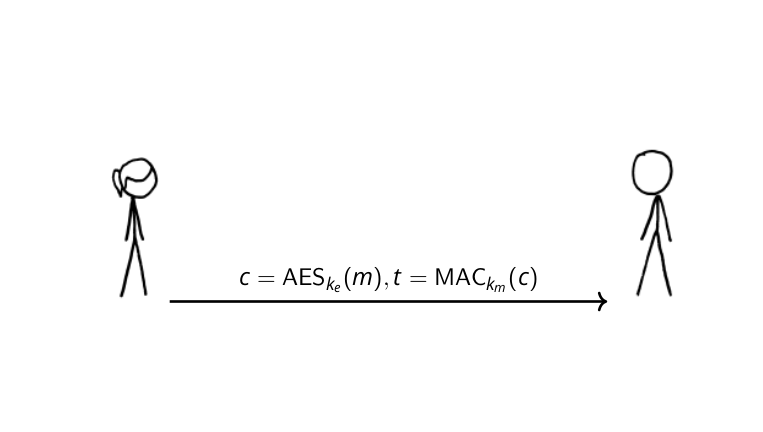
\includegraphics[scale=.7]{./tls1.png}
\end{center}

{\parindent0pt Alice (left) and Bob (right) want to communicate on a secure 
channel that is protected against passive easedroppers and man-in-the-middle
attacks.}

\bigskip
{\parindent0pt Assuming Alice and Bob have shared a set of keys, Alice sends her
AES ciphertext and the MAC of the ciphertext to Bob.  Bob can now check the MAC
and decrypt the cipher text to get the original message.}

\bigskip
{\parindent0pt The MAC is a short string of data which authenticates the message, i.e. it
confirms that the message was sent by the true sender and was not modified in transit.}

\subsection{Diffie-Hellman key exchange}
In order to negotiate charing encryption and MAC keys, there must be a
Diffie-Hellman key exchange.

\begin{center}
	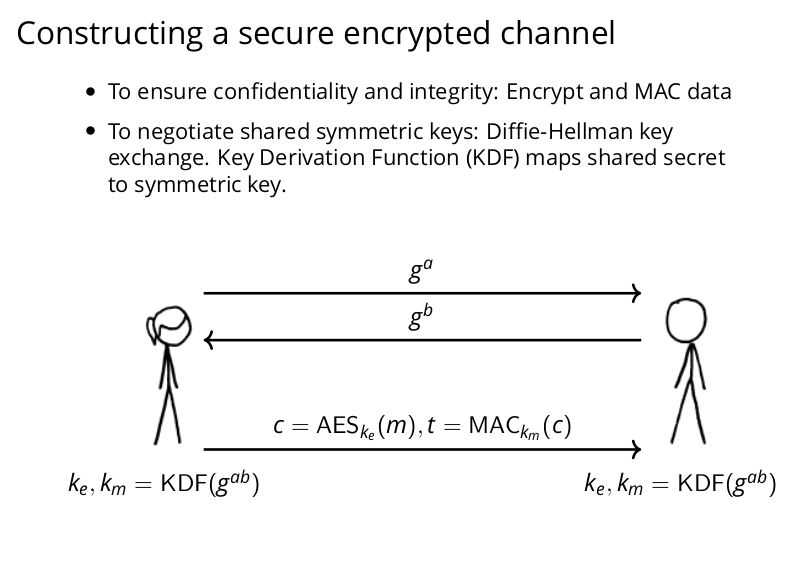
\includegraphics[scale=.7]{./tls2.png}
\end{center}

{\parindent0pt \textbf{Note:} In the image above $g^{a}$  should be read as 
$g^{a}\ mod\ p$ and likewise $g^{b}$ should be read $g^{b}\ mod\ p$}

\bigskip
{\parindent0pt If a Diffie-Hellman key exchange has occurred then both Alice 
and Bob will have a \textbf{shared secret}. In this case Alice and Bob's shared
secret is $g^{ab}$.}

\bigskip
{\parindent0pt Using this shared secret Bob and Alice can use a Key Derivation
Function (KDF), 
\smallskip
$k_e, k_m\ =\ KDF(g^{ab})$, which we can think of as a hash function that is 
used to create encryption and MAC keys they can use for symmetric cryptography.}

\subsection{Ensure Authenticity of Endpoints}
There is a vulnerabiliy with this approach because if there is an active
man-in-the-middle attack, the attacker can intercept the Diffie-Hellman
key exchange.  To ensure the authenticity of the endpoint we must use
\textbf{digital signatures}, to prevent man-in-the-middle interference of the
key exchange.
You can have either one or both parties sign the key exchange with a long-term
public key.

\begin{center}
	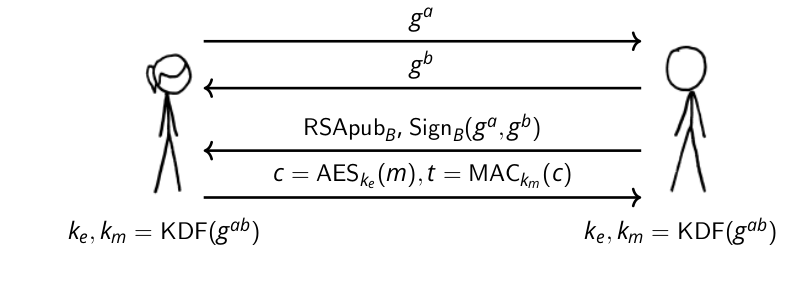
\includegraphics[scale=.7]{./tls3.png}
\end{center}

For example, assume that Alice is the client (web browser), Bob is 
the web server, Alice knows the server's long-term key, and Alice is trying to
communicate with Bob.

\bigskip
To protect the Diffie-Hellman key exchange Bob will sign the key exchange with 
his long-term key.  Since Alice knows both Bob's original long term-key and the
signature which Bob has given Alice, she can verify the signature by using Bob's
public key before progressing with the encryption.

\subsection{Trusting Signatures}
While we may now be protected against man-in-the-middle attacks targeted towards
the Diffie-Hellman key exchange, we have still not verified the integrity of
Bob's public signing key which Alice has received.

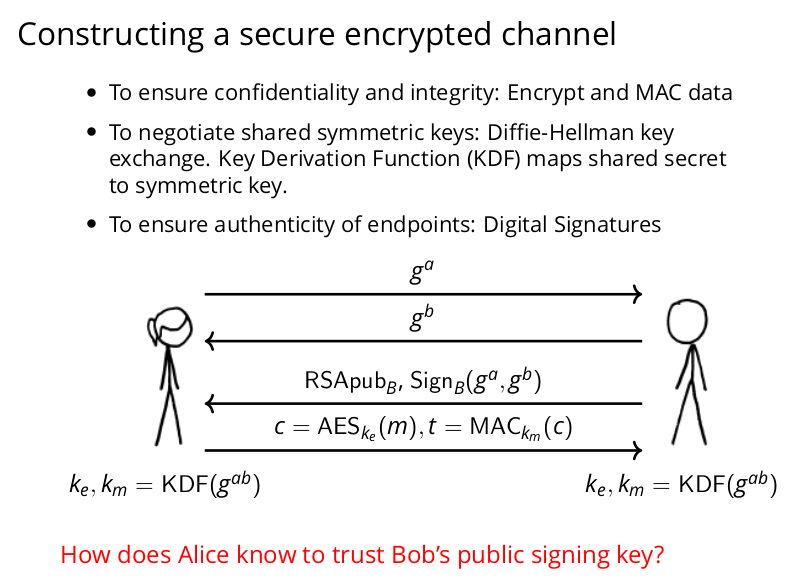
\includegraphics[scale=.7]{./tls4.png}

The public signing key that Bob sends to Alice is susceptible to
active man-in-the-middle attacks, so we must determine a way to trust the keys 
that the client receives.

\bigskip
Assuming that there is a man-in-the-middle who is intercepting all of the
communications between Alice and Bob, an attacker can substitute Bob's public
key with their own generated public key and Alice would not be able to tell 
the difference.

\bigskip
Due to the nature of this attack, we must have an \textbf{external} method of
establishing trust in keys.

\subsection{Establishing Trust in Keys}
Ways to establish trust in keys:
\begin{itemize}
  \item Meet in person to exchange keys.
  \begin{itemize}\item This is the simplest way, however this is not practical at scale over the internet
  \end{itemize}
\end{itemize}



\begin{itemize}
  \item Fingerprint verification.
  \begin{itemize}\item This is used by SSH for host keys.  \item verify a cryptographic hash of a public key through a separate channel or “Trust On First Use” (TOFU). 
  \end{itemize}
\end{itemize}

If you think that your connection probably hasn't had a man in the middle the first time that you connect, then you can trust that forever. If that ever changes, you get a warning message.

\begin{itemize}
  \item Hard code public keys in software
  \begin{itemize}\item “Certificate pinning” used by browsers to protect against attacks: "certificate pinning" bakes in keys into software.
 
  \end{itemize}
\end{itemize}

\begin{itemize}
  \item Certificate Authorities
  \begin{itemize}
  \item A certificate authority (CA) is  a kind of commercial trusted intermediary that verifies public keys and signs them in exchange for money. This is used for TLS, software signing keys. 
  \end{itemize}
    If you trust the Certificate authority, you transitively trust the keys it signs. The CA can't decrypt your traffic because all they are doing is signing the public key, and they never see the private key.
\end{itemize}


\begin{itemize}
  \item  Web of Trust

  This is an alternative to trusting commercial companies: you trust your friends because you can't meet everybody, but if your friends have met somebody and signed their public key, you can also trust that person. Anybody who trusts my public key will trust x’s.
  \begin{itemize}
  \item This is used by PGP.

  PGP (Pretty Good Privacy) is an email encryption open source program written in the early 1990s . It is very difficult to use it: you must install a key base, which hides details of cryptography. The key base acts as a trusted third party to store your public keys along with your identity. Other options for doing PGP is using the command line tool. The image below is an example of using command line tool.
\bigskip

\begin{center}
	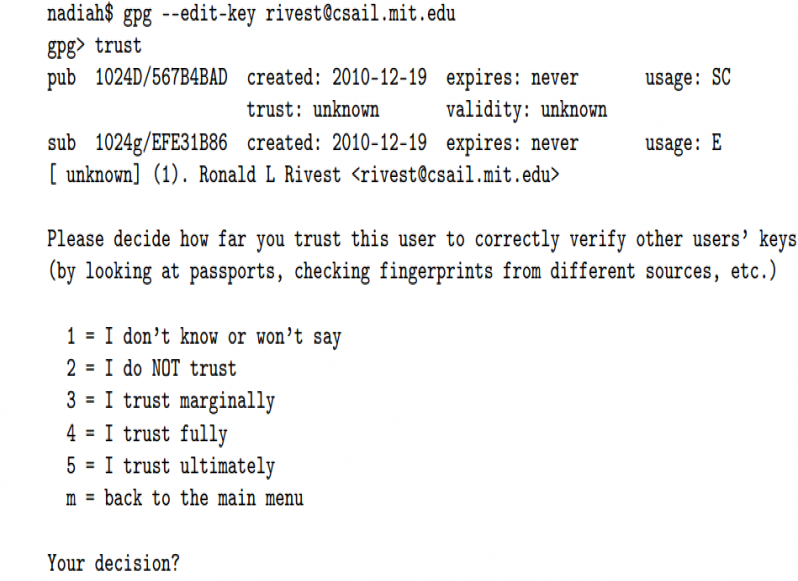
\includegraphics[scale=0.55]{./Trust-in-keys2.png}
\end{center}
 
  \end{itemize}
  
  
\subsection{Using RNG in Signature}

Returning our discussion to the secure channel: assume Alice knows to trust a key because it has a certificate authority signature or it is baked into our software. Now Alice and Bob are able to negotiate a fresh shared session key and encrypt all of their messages using symmetric crypto which will be secure against an active man in the middle and a passive eavesdropper.\\

{\parindent11pt One final detail: in order to protect against an adversary from replaying a signature (reusing it across multiple handshakes), you might include some extra randomness, for example a nonce, a value that you use once. It doesn't necessarily have to be cryptographically strong, but it has to be unpredictable to 
the adversary. The signature is over these randomly chosen values so should be different every time the protocol runs, so adversaries can't steal the signature from a previous protocol.}

  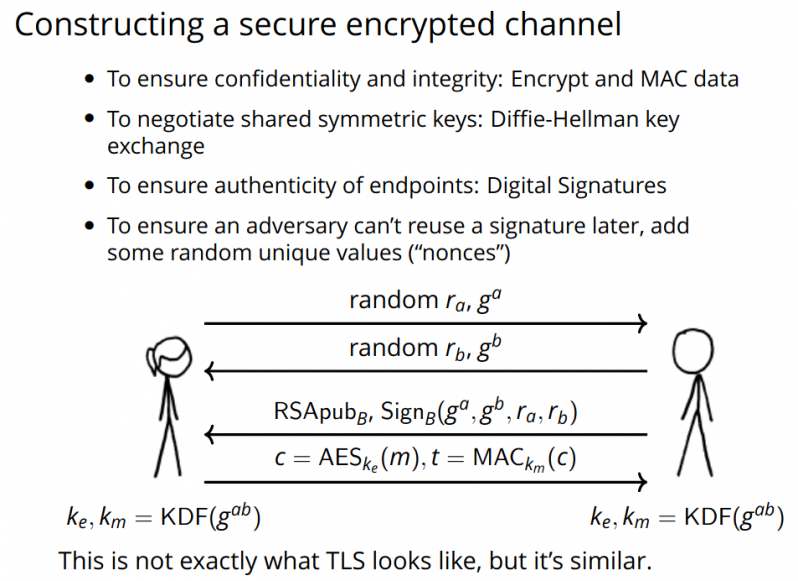
\includegraphics[scale=0.6]{./Trust-in-keys3.png}

Keep in mind that the Diffie-Hellman key exchange is subject to a man in the middle attack. Therefore you need to use digital signatures, because you need to know where to get your trust from the public key that is signed, so you need a public key infrastructure. Once you've done that, then you can trust that Diffie-Hellman key exchange hasn't been man in the middle. Then you derive symmetric session keys and then use symmetric crypto to encrypt the content.

\end{itemize}

\section{TLS: Transport Layer Security}

\subsection{TLS Overview}
TLS was called SSL in the 1990s. It provides an encrypted channel for application data. It's used for HTTPS (HTTP inside of a TLS session). Keep in mind that the content that's being sent, like the symmetrically encrypted messages, once negotiation is done, is like the HTTP connection. There are several protocol versions which are not numbered sequentially. 
Academic papers show that maintaining support for old versions of the protocol lead to bad downgrade and decryption attacks.

\begin{itemize}
\item SSL 1.0 Terribly insecure; never released.
\item SSL 2.0 Released in 1995; terribly insecure,deprecated in 2011.
\item SSL 3.0  Released in 1996; terribly insecure,deprecated in 2015.
\item TLS 1.0 Released in 1999; deprecated in 2020. 
\item TLS 1.1 Released in 2006; deprecated in 2020.
\item TLS 1.2 Released in 2008. Ok.
\item TLS 1.3 Standardized in August 2018 and is being rolled out now;  major change from TLS 1.2 .
\end{itemize}
TLS 1.1, 1.2,  and 1.3 are similar, but in general TLS 1.3 is a better protocol. Older versions of TLS have potential flaws.

\subsection{TLS 1.2 with Diffie-Hellman Key Exchange}

\subsubsection{Step 1}
\begin{center}
	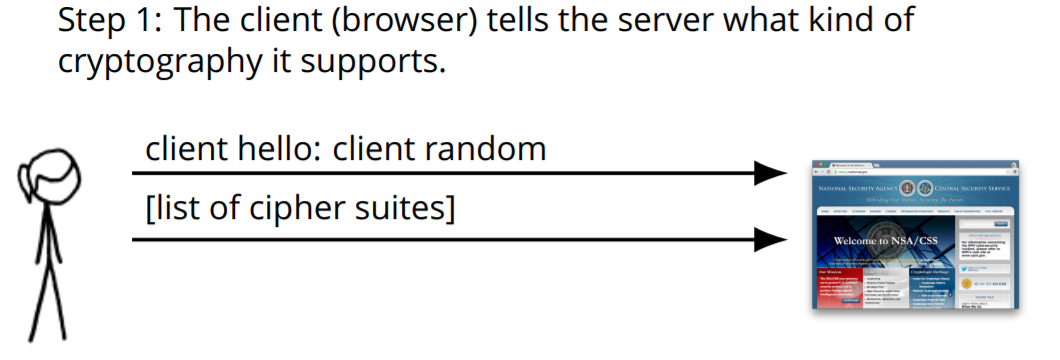
\includegraphics[scale=.5]{./DiffieStep1.png}
\end{center}

\subsubsection{Step 2}
\begin{center}
	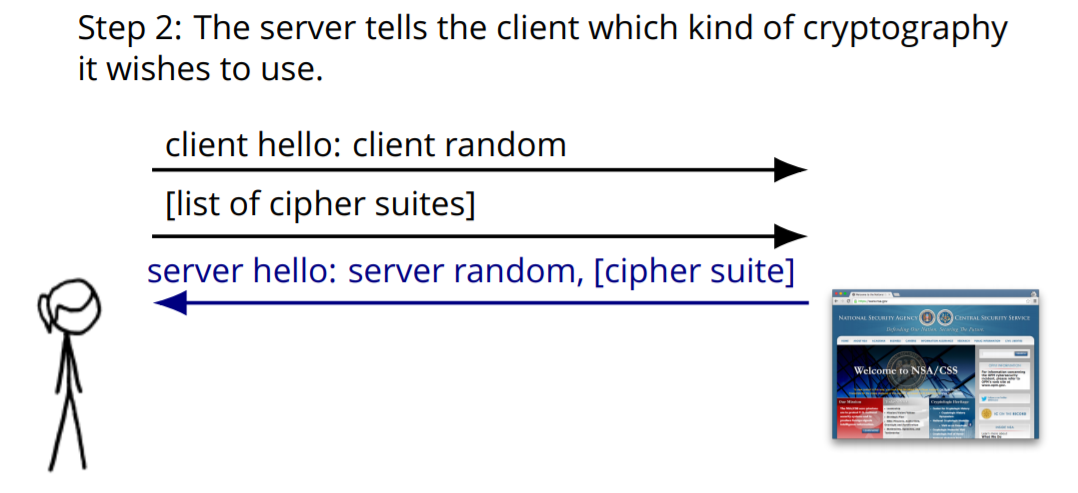
\includegraphics[scale=.5]{./DiffieStep2.png}
\end{center}

\subsubsection{Step 3}

\begin{center}
	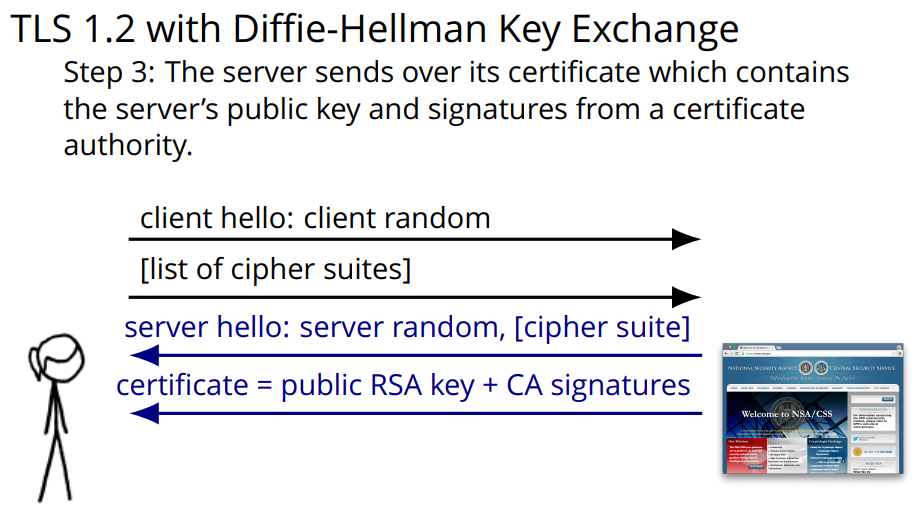
\includegraphics[scale=.8]{./DiffieStep3.png}
	\\(Certificates are explained more in Section 3.3)
\end{center}

\subsubsection{Step 4}

\begin{center}
	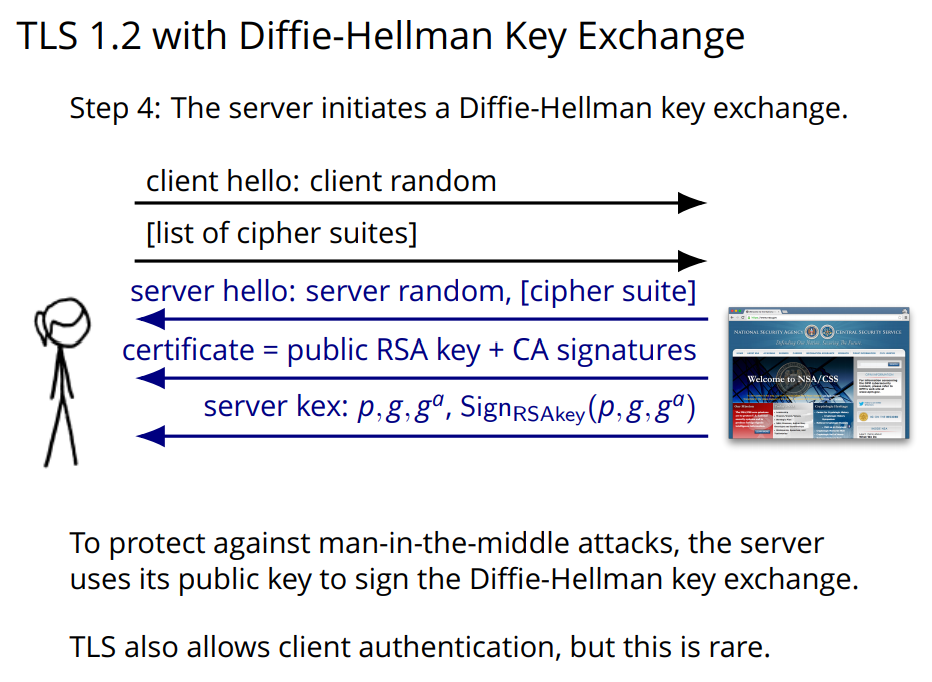
\includegraphics[scale=.8]{./DiffieStep4.png}
\end{center}

 \noindent The server will sign its part of the key exchange, shown as 
 $Sign_{RSAkey}(p,g,g^a)$ in the image above. Since the message is signed by 
 the server's RSA key, which is signed by a certificate authority that Alice 
 trusts, it cannot be modified by a man-in-the-middle attack.

\subsubsection{Step 5}

\begin{center}
	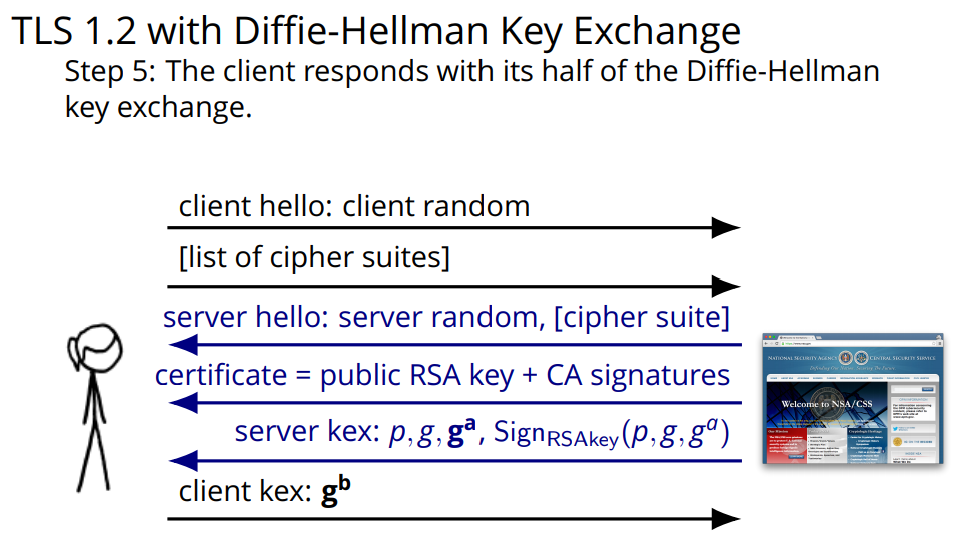
\includegraphics[scale=.8]{./DiffieStep5.png}
\end{center}

\noindent This message is usually not authenticated since user authentication is not 
commonly done at the cryptographic layer when using the web.

\subsubsection{Step 6}

\begin{center}
	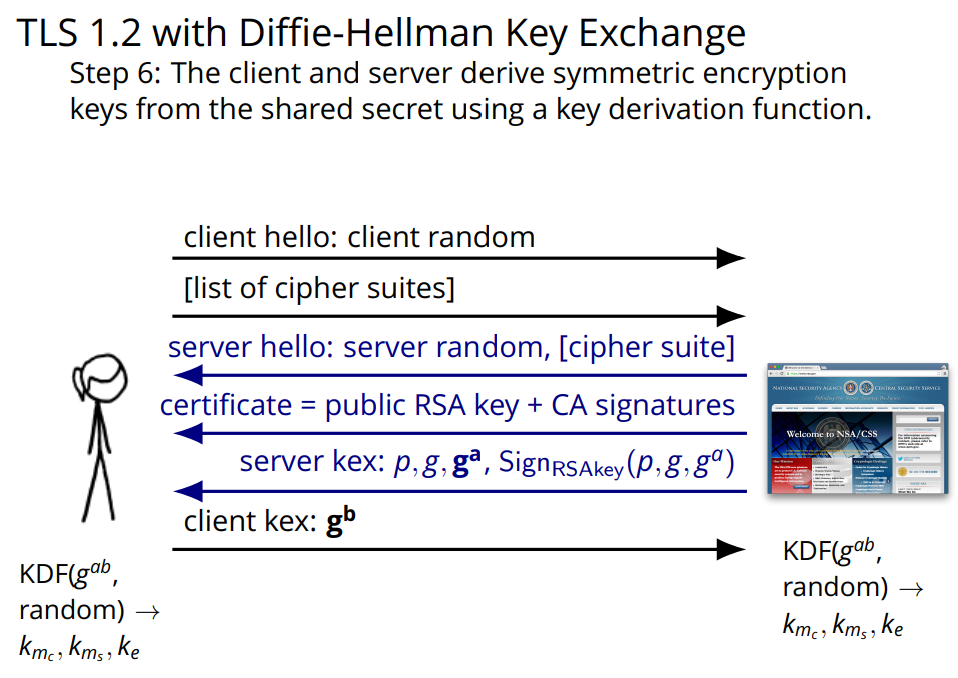
\includegraphics[scale=.8]{./DiffieStep6.png}
\end{center}

\noindent $KDF$ is the key derivation function,
$k_{m_c}$, $k_{m_s}$, and $k_{e}$ are the symmetric keys,
$k_{m_c}$ is the client's MAC key, $k_{m_s}$ is the server's MAC key and $k_{e}$ 
is the encryption key.

\subsubsection{Step 7}

\begin{center}
	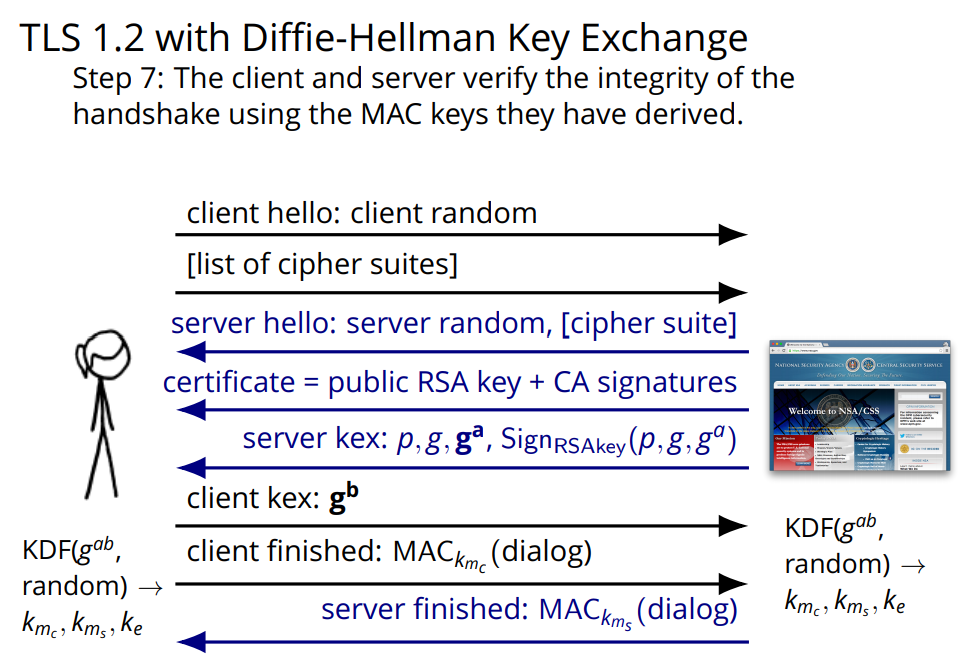
\includegraphics[scale=.8]{./DiffieStep7.png}
\end{center}

\noindent They can verify the integrity of the handshake by each sending a MAC (Message 
Authentication Code) of all of the messages they have sent so far using the 
symmetric keys that they derived in the last step. This guarantees that the channel is secure.

\subsubsection{Step 8}

\begin{center}
	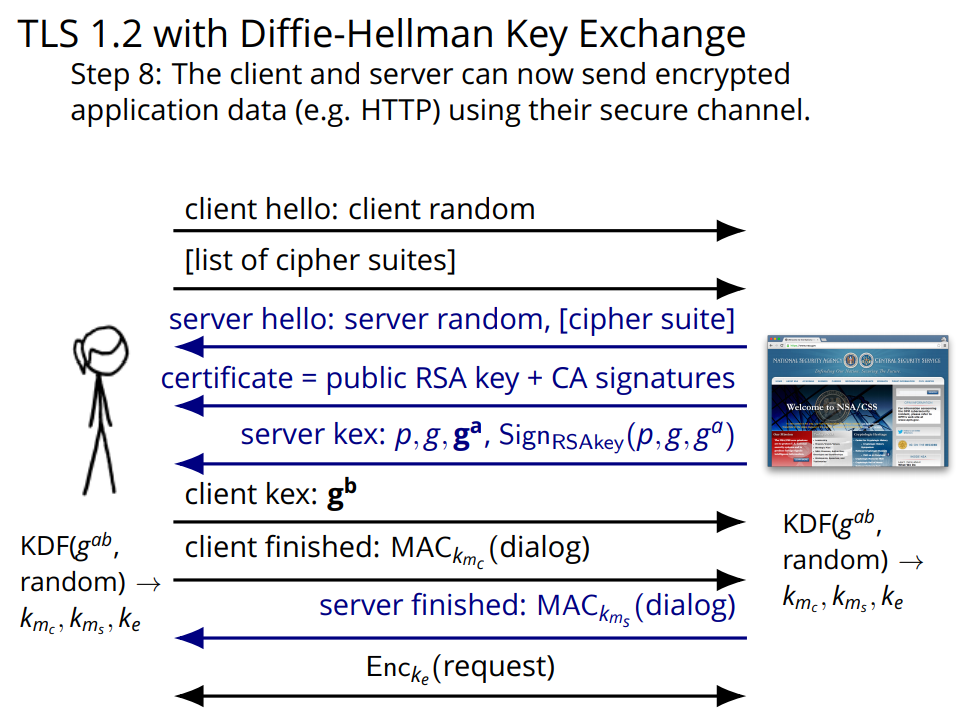
\includegraphics[scale=.8]{./DiffieStep8.png}
\end{center}

\noindent For example, Alice (client) will make an HTTP GET request for index.html over 
the encrypted channel.

\subsection{Certificates and Certificate Authorities in TLS}
\begin{figure}[H]
    \centering
    \textbf{Sample Certificate}\par\medskip
    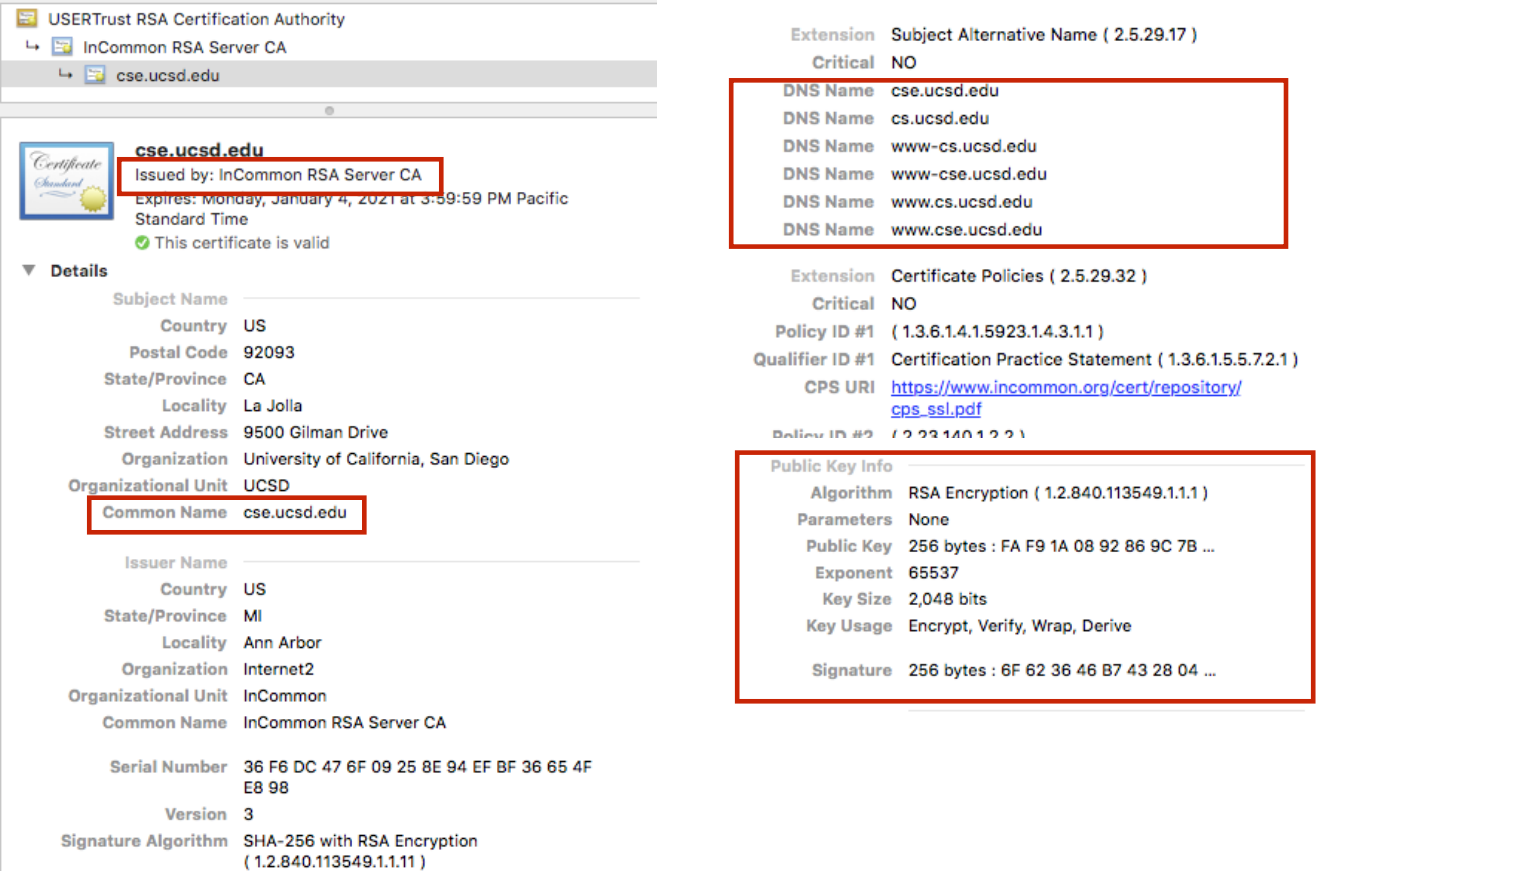
\includegraphics[scale=.4]{./cert1.png}
    \caption{an example of a valid certificate from cse.ucsd.edu}
\end{figure}
\begin{itemize}
      \item  The certificate authority (CA) is InCommon RSA Server CA.
      \item The domain name for which this certificate is meant is cse.ucsd.edu, with multiple DNS names listed
      \item The public key uses RSA Encryption, with exponent 65537, N = 2048, and the public key and signature are both view able to the user.
\end{itemize}

\begin{figure}[H]
    \centering
    \textbf{Sample Certificate Cont.}\par\medskip
    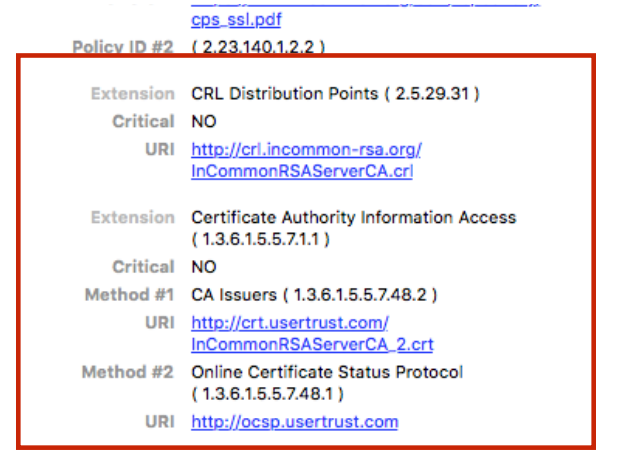
\includegraphics[scale=.5]{./cert2.png}
    \caption{This part of the certificate tells the user where to look for revocation information}
\end{figure}


\subsection{Revocation}
It's possible for a key to be compromised, ie for an attacker to obtain a private key. This is clearly undesirable, as any private/encrypted messages sent to whomever owns this private key can now be read by the attacker, and/or the attacker can sign any messages he wants as if he were the original owner of the private key. In the case that a Certificate Authority key is compromised, a client may receive a perfectly valid certificate that was signed by an attacker, and there would be no way of knowing this certificate is invalid unless the CA announced that their public key is no longer valid.

\bigskip
Therefore, there exists a revocation process for public keys. If Alice, for example, finds out that her private key has been compromised, she is able to announce or allow her senders to find out that her public key is no longer valid and they should not be using that public key to encrypt messages to her anymore. This verification must be signed by the private key, as you wouldn't want anyone else to arbitrarily cancel your key. Both CA and PGP PKIs support this. 
\begin{figure}
    \centering
    \textbf{Compromised Certificate: Man in the Middle}
    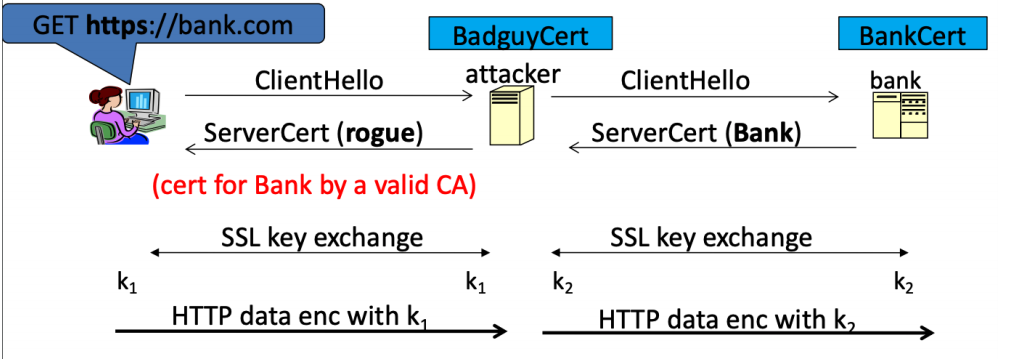
\includegraphics[scale=.4]{./cert3.png}
    \caption{Man-in-the-middle attack using rogue certificate}
    \begin{itemize}
      \item The attacker has managed to obtain valid certificates from a CA trusted by the client.
      \item This allows the attacker to intercept the data being sent from the bank, and send the client his own "certified trusted" public key as if he were the bank; the client will accept this, (since it has the valid certificate) encrypt her data using this malicious key, and send the data to the bank.
      \item This gives the attacker free reign to proxy any and all traffic to and from the client and the bank, modifying any data as he pleases, as he can decrypt whatever the client was sending to the bank.
      \item One could imagine the attacker modifying the client request to say something along the lines of "transfer all the money to the attacker account." 
    \end{itemize}
\end{figure}

\subsection {CA Hacks / Vulnerabilities}
\paragraph{There is a long history of CAs getting hacked or certifying wrong things}
 \begin{itemize}
    \item 2011: Comodo + DigiNotar hacked to issue fraudulent certificates for Hotmail, Gmail, Skype, Yahoo Mail, Firefox
    \item 2013: TurkTrust issued fraudulent certificate for Gmail
    \item 2014: Indian NIC issue certs for Google and Yahoo!
    \item 2016: WoSign issues cert for GitHub.
\end{itemize}
\paragraph{Mitigations}
\subparagraph {Certificate pinning:} Limits risk by restricting which certificates are considered valid for a particular website. Instead of allowing any CA in the trusted list to sign a certificate, the browser pins the CA of choice; any certificates received that are not from this pinned CA are considered invalid. Therefore, attackers are unable to man in the middle even if they have a valid certificate from a trusted authority as long as the pinned authority doesn't match.
\subparagraph {Certificate Transparency:} All certificates are publicly disclosed, providing greater insight and transparency. Certificate transparency has two main components, logs and monitors.
 \begin{itemize}
    \item Logs maintain records of all issued certificates to a domain. These logs are append only, and cannot be altered or deleted once a certificate has been added to the log (using something called a Merkle Tree to achieve this)
    \item Monitors do just that, monitor the logs for anything they can be set to monitor. Some monitors can allow users to create and run queries for certificates, as google does. Some domains may be interested in receiving notifications for when a certificate is issued to their domain, or if it matches some query they are interested in monitoring.
\end{itemize}

\subsection{TLS 1.2 with RSA Key Exchange}
Another way to negotiate keys in TLS 1.2 is using RSA public key encryption to 
share a secret master key.

\begin{enumerate}
  \item This starts with the Alice[client] sending a hello.
  \item Then, the server will send over its certificate, which contains its 
  public key.
  \item Alice[client] will choose a random value, called a premaster secret, 
  which she encrypts to the server's RSA public key and sends back to the 
  server.
  \item The server is the only one who can decrypt the value of the encrypted 
  premaster secret.
  \item The server and client will then use a key derivation function to 
  derive their encryption and MAC keys.
  \item The server and client will exchange MACs of the dialogue.
  \item Finally, they will send encrypted requests using the symmetric 
  encryption key.
\end{enumerate}

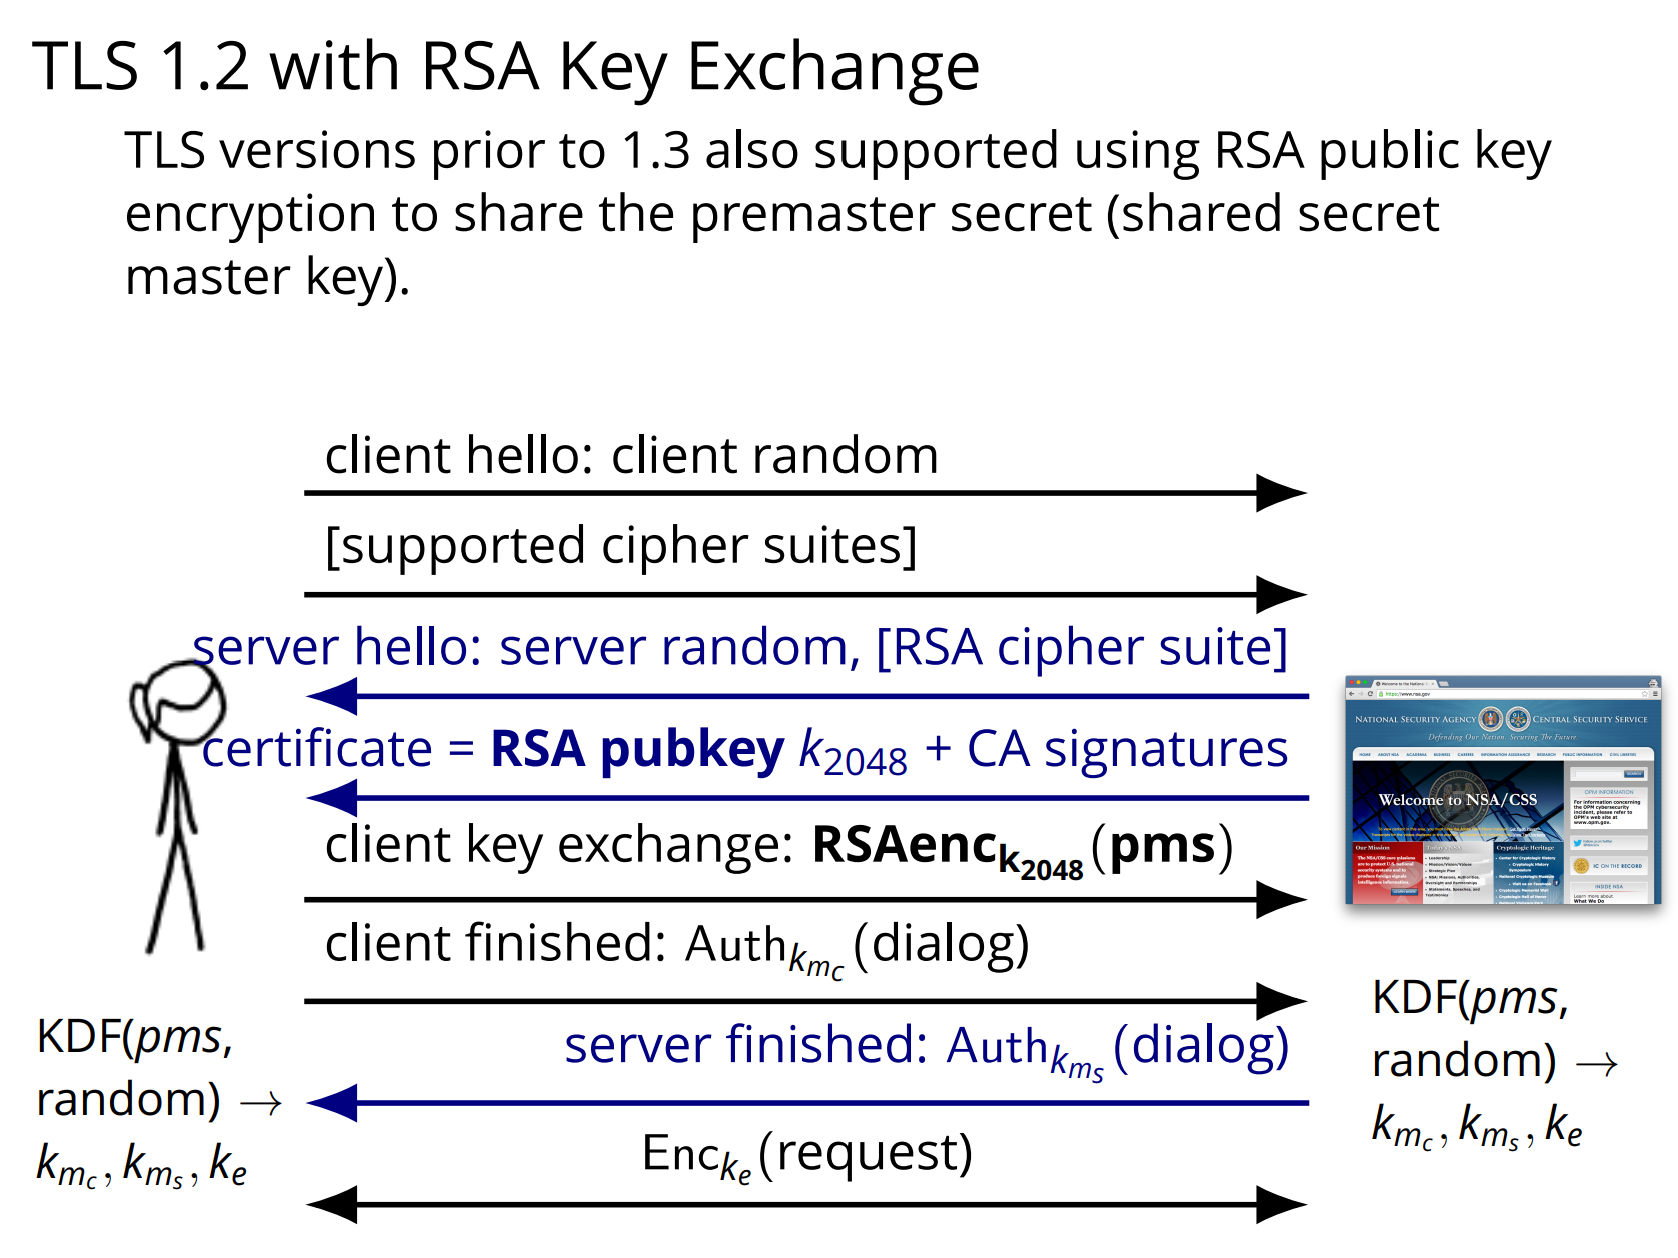
\includegraphics[scale=.6]{./TLS_RSA.png}

The only difference from using the Diffie-Hellman key exchange is the client 
instead encrypts a secret and sends it to the server.

\subsection{How TLS Achieves Its Security Goals}
It allows transmitting information between a client and the server with an encrypted connection. Listening in, only allows the recipients who are exchanging information to be seen. Without the secret keys the information cannot be decrypt it.
\subsection{What If a Private Key Gets Stolen or Compromised?}
\begin{itemize}
  \item The attacker is able to actively man-in-the-middle a connection. Therefore, they are able to impersonate the server to others. This allows the attacker to eavesdrop between the parties. With the a valid secret key they are able to decrypt messages that are being sent from the users compromised key.
  \item With a compromised RSA key, the attacker can obtain the session keys and decrypt the sessions information. Any past traffic that is recorded can also be decrypted with such an attack.
\end{itemize}
\subsection{TLS v. 1.2 and Below Vulnerabilities}
\begin{itemize}
  \item TLS 1.2 and below allowed attackers manipulate data between client and servers. Including credit card information, credentials, and other valuable information. 
  \item TLS 1.2 addressed these concerns. They allowed clients and servers to choose specific hash and signature algorithms. Allowed authenticated ecryption for other data modes.
  \end{itemize}

\subsection{TLS 1.3}
\begin{itemize}
  \item Removes the support of SHA-224 and MD5 because of the compromised vulnerabilities. 
  \item Removes RSA key exchange, which allowed protection for passive decryption
  \item Allowing handshake encryption immediately after key exchange. This limits the amount of data that an eavesdropper can see. Also a noticeable slower time to secure a connection.
\end{itemize}

\subsection{TLS Key Theft and Other Risks in the Wild}
\begin{itemize}
  \item A very common attack is SSL tripping. The attacker gets in between the user and an encrypted host. They act as a middle host between the client and secured website. Any information the user enters will first go through the attacker
  \item Using expired TLS certificates can cause a man-in-middle attack. Therefore, any expired certificates should be removed from servers.
 \item Not identifying any forges or untrusted certificates
\end{itemize}

\subsection{The “Crypto Wars” and the Historical Development of TLS}
\begin{itemize}
  \item Unofficial term used to describe the feud between governments and their attempt to limit the access cryptography strong enough to go unrecognized by intelligence agencies. In 1975 the U.S. introduced the Data Encryption Standard, but led many to believe there will always be a back door if a government wanted to eavesdrop on "encypted" data.
  \item The development of TLS has been supported by governments in order to keep secure connections between clients and servers, while keeping with government standards.
\end{itemize}

\subsection{TLS Keytheft and Other Risks in the Wild}
If an attacker was able to issue validated certificates for a domain they don’t own, then they wouldn’t need to get a hold of any existing private keys. They would just make their own key pair and issue a certificates for it. The attacker DoS’s the victim’s server and stands their own server up using the attacker’s certificate and key.
\\
However, if an attacker gets the private key for a victim’s server then the attacker does not need to create a new certificate. The attacker will just grab the existing cert (it’s already being handed out by the victim’s server) and DoS the victim’s server and stand up their own server using the victim’s cert and key.
\\
Often an ordinary user is vulnerable to one or more parties that they don't really trust, between them and any particular peer out on the Internet, this might be the proprietor of the coffee shop where they're using WiFi, or their home ISP, the network engineers at their employer's place of business, or even the sovereign government of the country they're in.

\subsection{Lavabit}
Even if TLS and key exchange works perfectly, there is still the matter of old-fashioned extortion by powerful governments. For example, consider the events of 2013 after Edward Snowden blew the whistle on the NSA's domestic spying capabilities.
Snowden was using a secure mail service Lavabit. In order for the US government to spy on his communications after his defection. Lavabit was commanded to appear in court, and to bring all of their TLS, HTTPS, and SSL keys to present to the court. However, Ladar Levison chose to bring a blurry, illegible photo which he claimed to be the TLS key.
\begin{center}
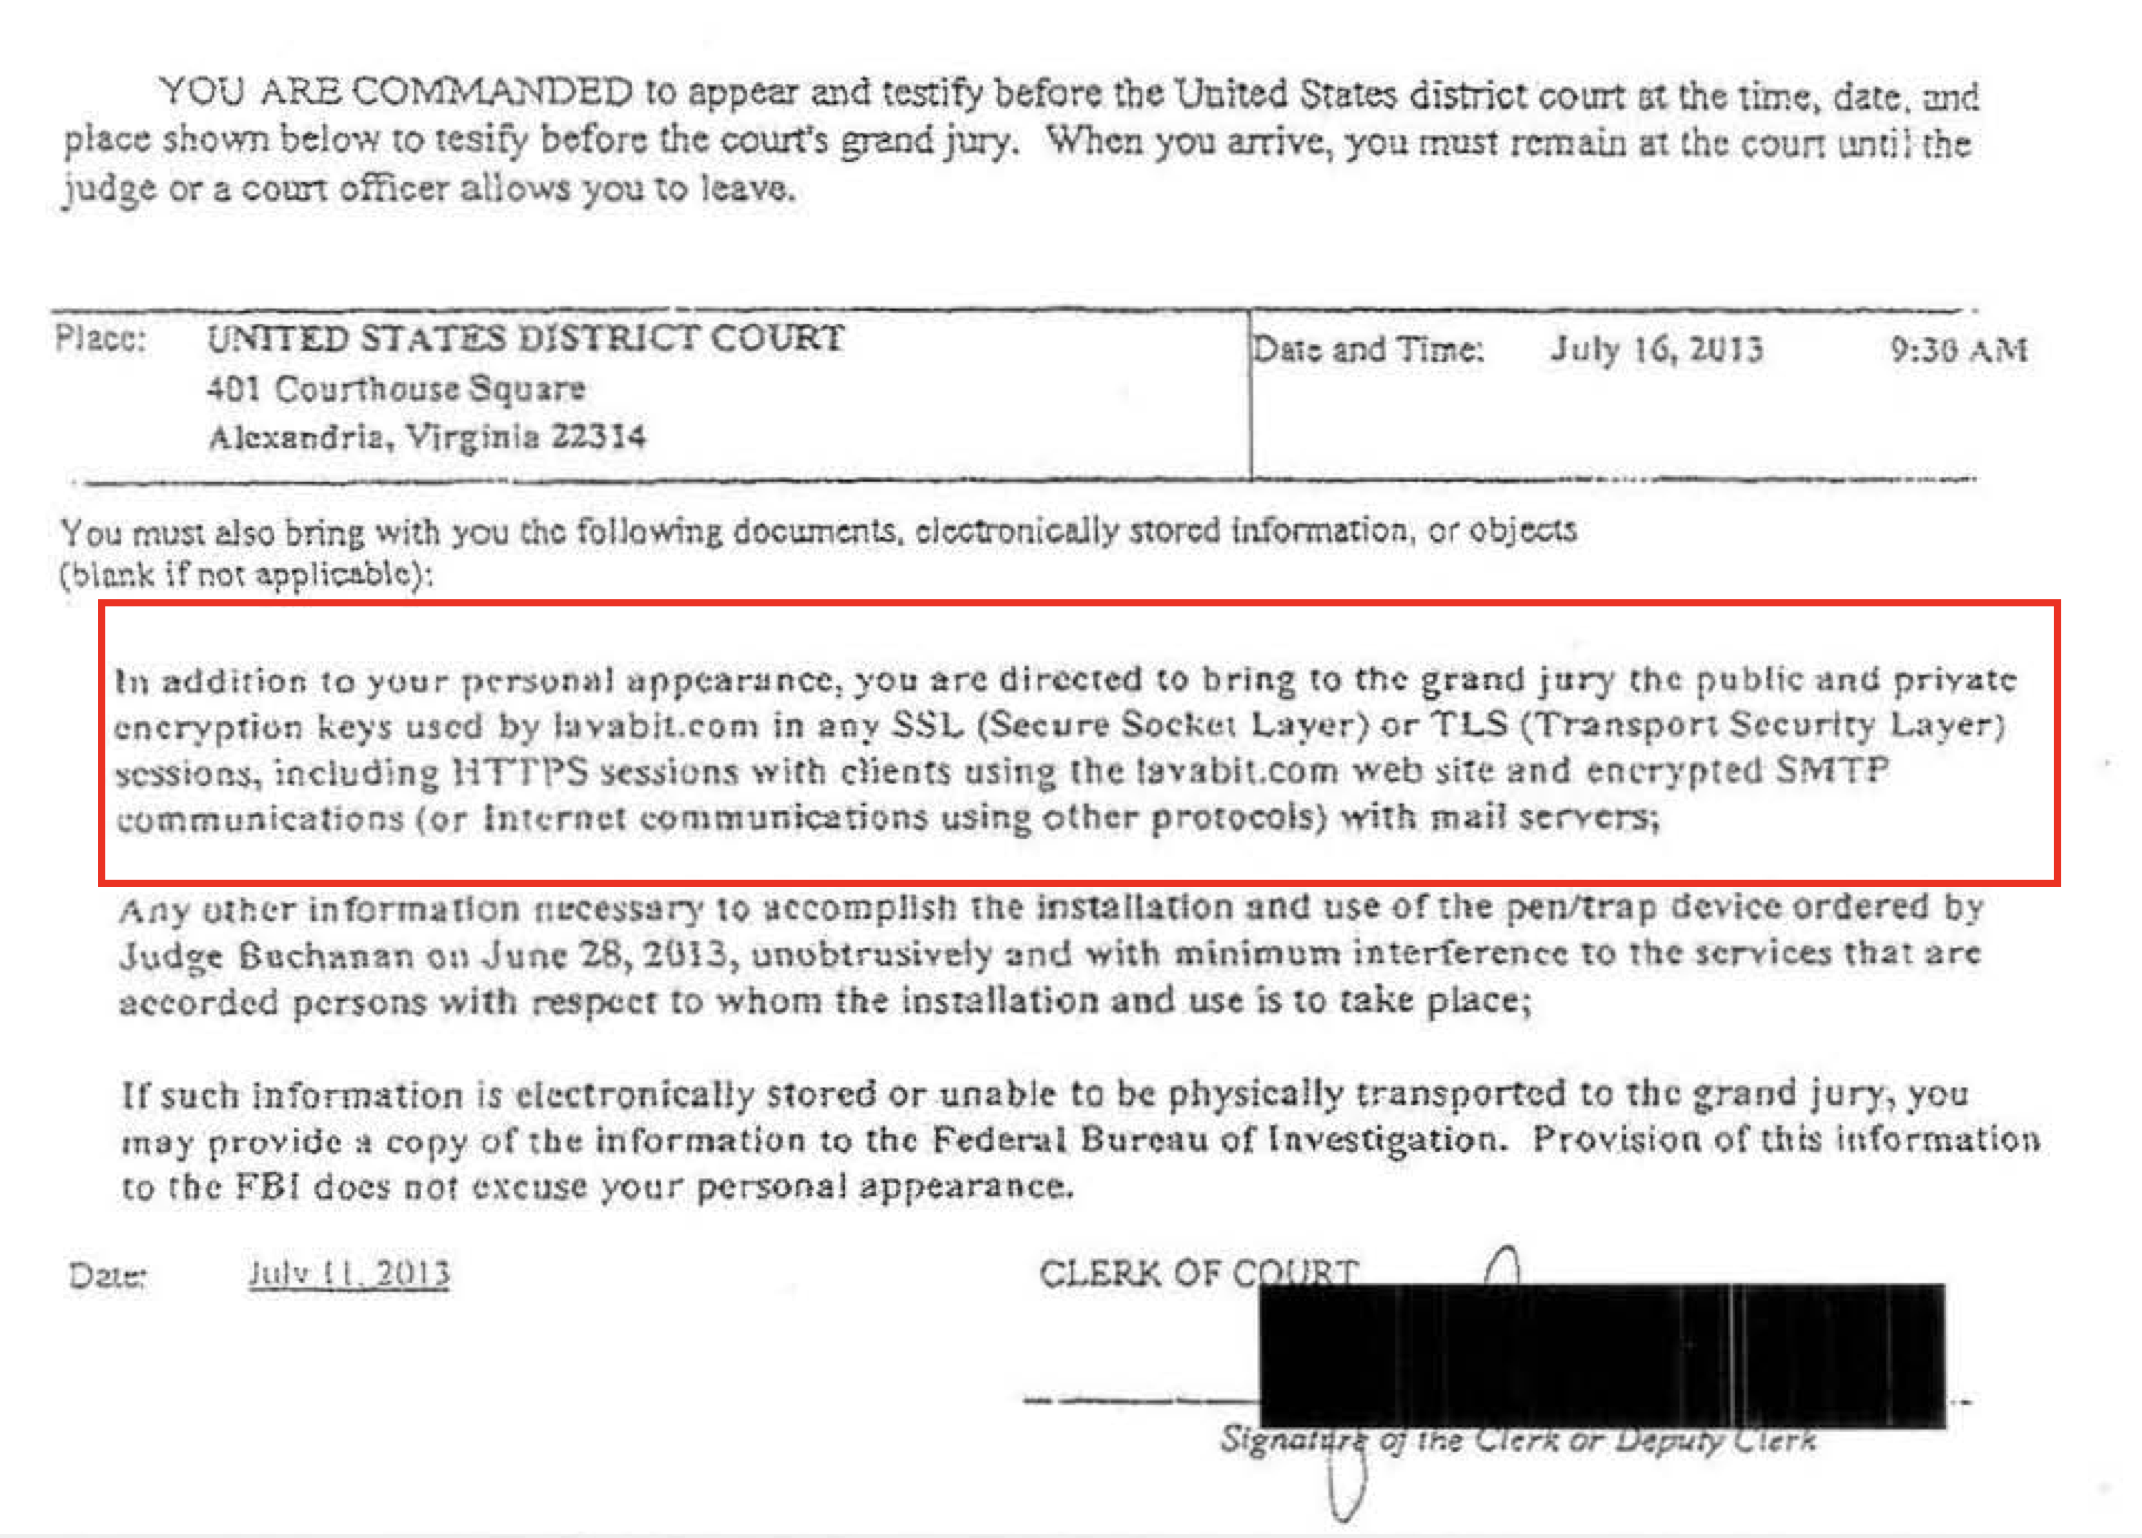
\includegraphics[scale=.3]{./lavabit-summons.png}
\\Lavabit summons
\end{center}

Lavabit never gave up the key, and instead chose to end their business operations rather than violate the privacy of their customers around the globe. Politicians and the US government do not care about the individual's right to privacy. For example, here is a quote from former president Barack Obama:

\begin{center}
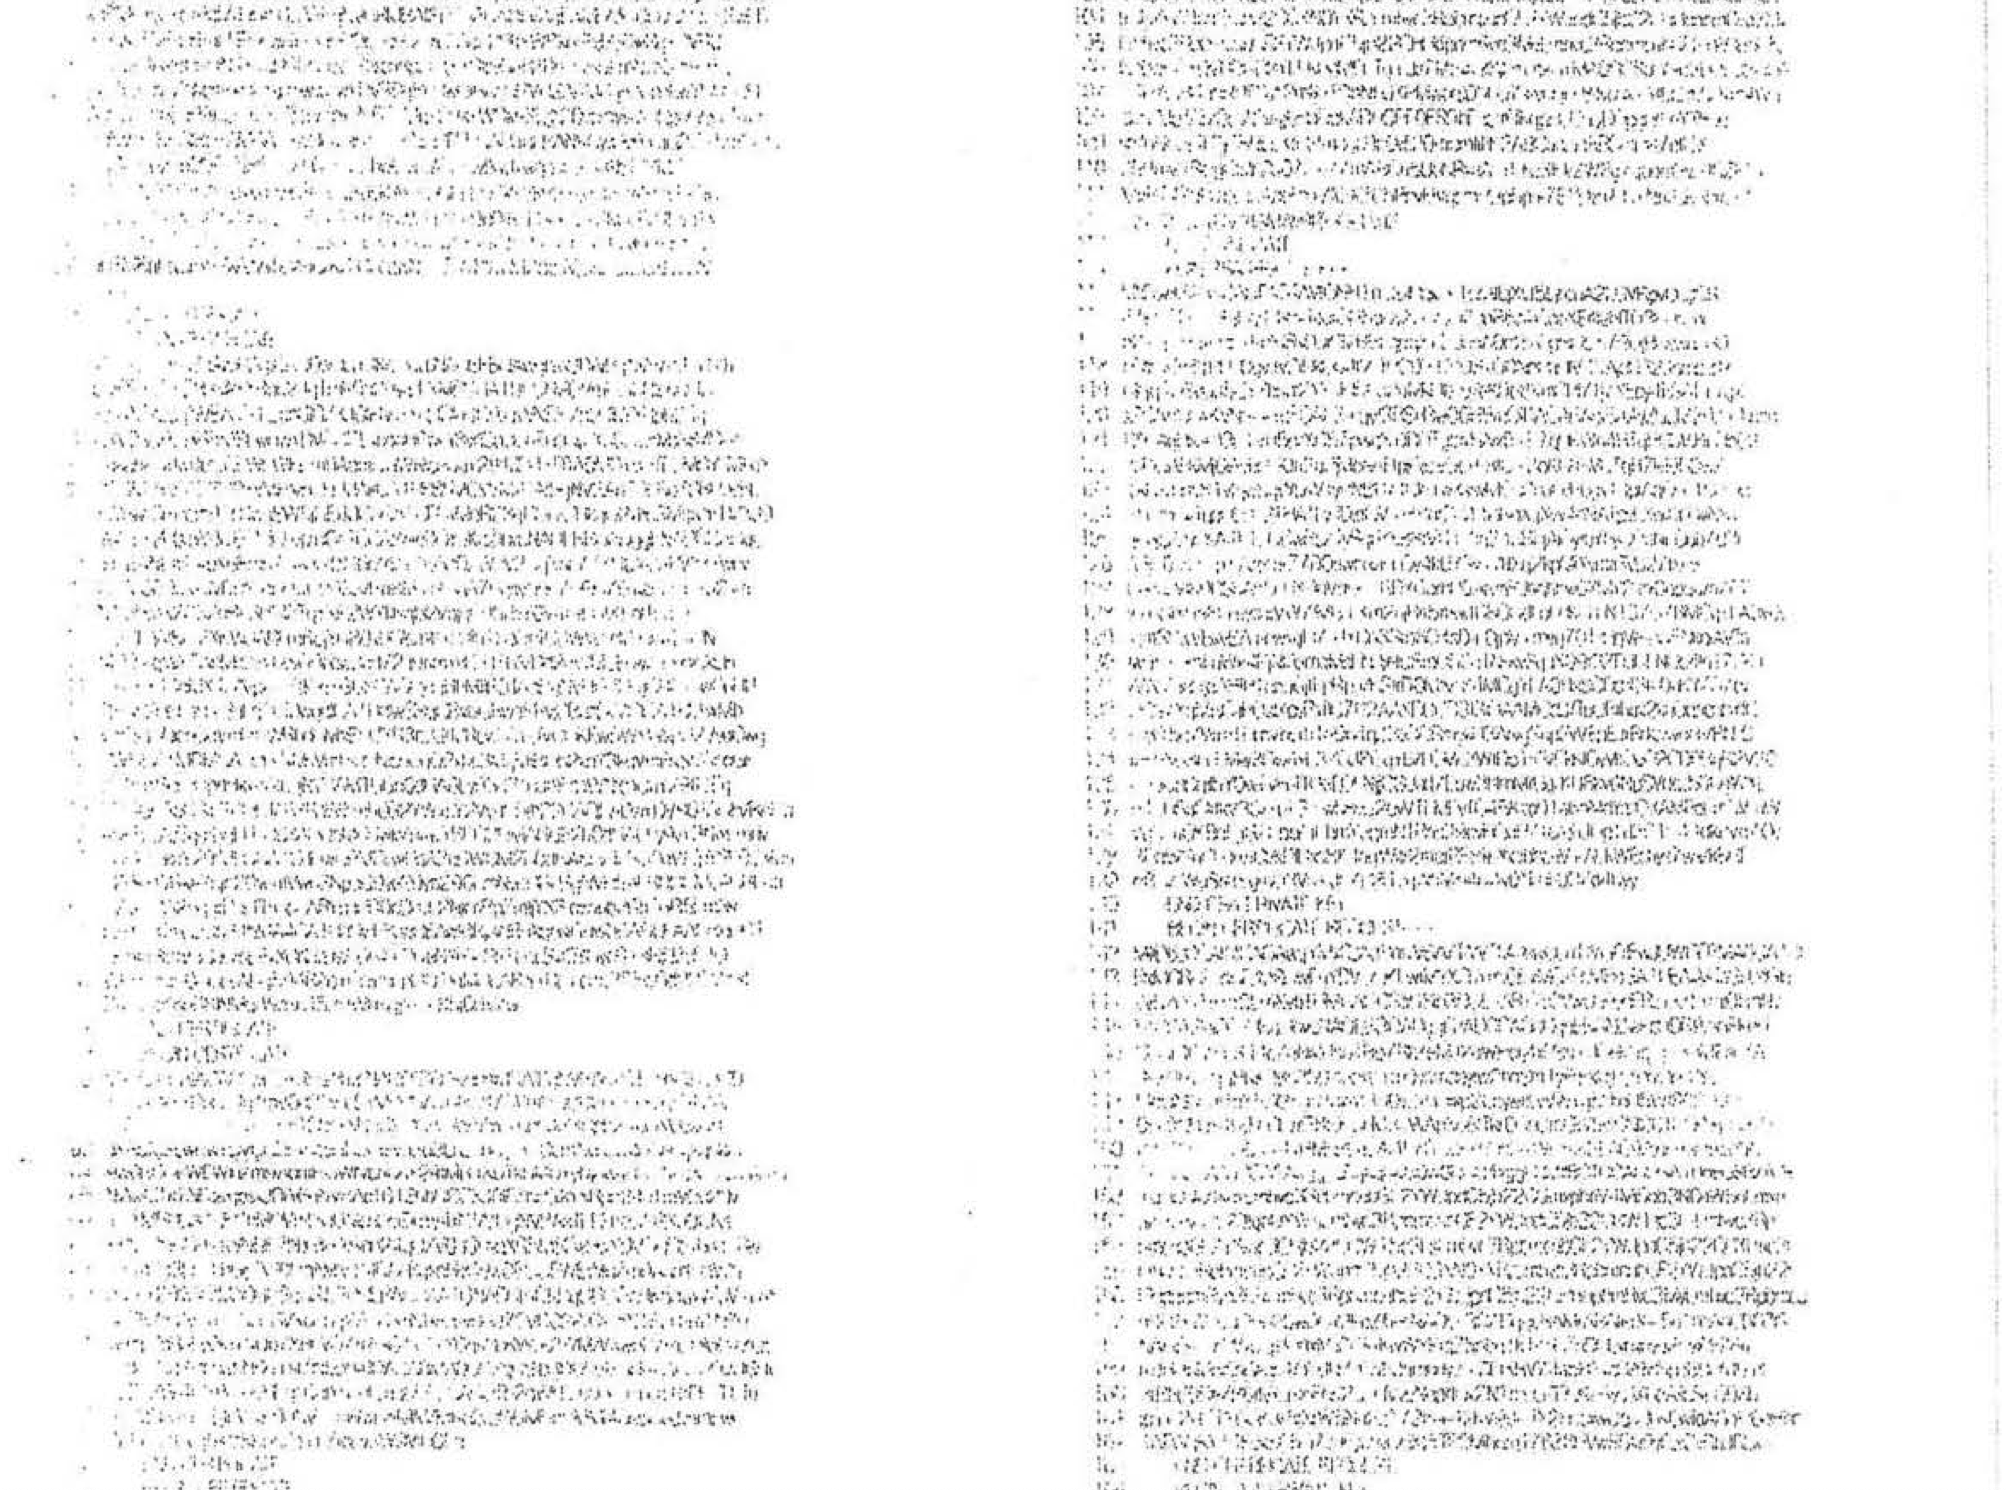
\includegraphics[scale=.3]{./lavabit-blurry-key.png}
\\The image of the key brought into court
\end{center}

"Because, if, in fact, you can’t crack that [encryption] at all, government can’t get in, then everybody is walking around with a Swiss bank account in their pocket – right? So there has to be some concession to the need to be able to get into that information somehow."


It is with this spirit that the US government has actually weakened encryption to make their job of spying easier. For example, in the 1990s, TLS 1.0 included options to weaken the protocol for US export control (browsers outside of the US were to request the weakened option). Even though these options are no longer required due to political shifts, there are still servers that respect the request. This lead to a series of attacks such as FREAK, logjam, and DROWN. 

\end{document}
